\section{Comportamento del Sistema}
\subsection{Descrizione della Rete di Petri} \label{PN-part1}
% Descrizione del comportamento del sistema (ad un certo livello di astrazione)
% utilizzando Reti di Petri.
Il comportamento del sistema è stato modellato, ad un certo livello di astrazione, utilizzando una Rete di Petri.
\begin{question}[Rete di Petri]
Una Rete di Petri è un approccio grafico alla rappresentazione dei sistemi ad eventi in cui è possibile che alcuni eventi occorrano concorrentemente. Si tratta di un modello formale astratto del flusso di informazioni, descrive ed analizza il flusso di informazioni del sistema.
\end{question}
Il flusso di controllo inizia dalla piazza \textit{start}, l'unica transizione attiva è \textit{initialize}.\newline Vengono inseriti dei token nella piazza \textit{threads}, i quali rappresentano i thread che l'applicazione può utilizzare.
Vengono inoltre identificati i documenti da elaborare e per ognuno viene inserito un token nella piazza \textit{documents}.
Si procede quindi nel trasformare tutti i file in task (\textit{ComputeDocumentTask}).\newline
Una volta creati tutti i task è necessaria la presenza di almeno un token nella piazza \textit{threads} per poter accedere alla piazza \textit{execute task}.
\begin{figure}[H]
    \caption{Rete di Petri del sistema utilizzando un approccio a task}
    \centering
    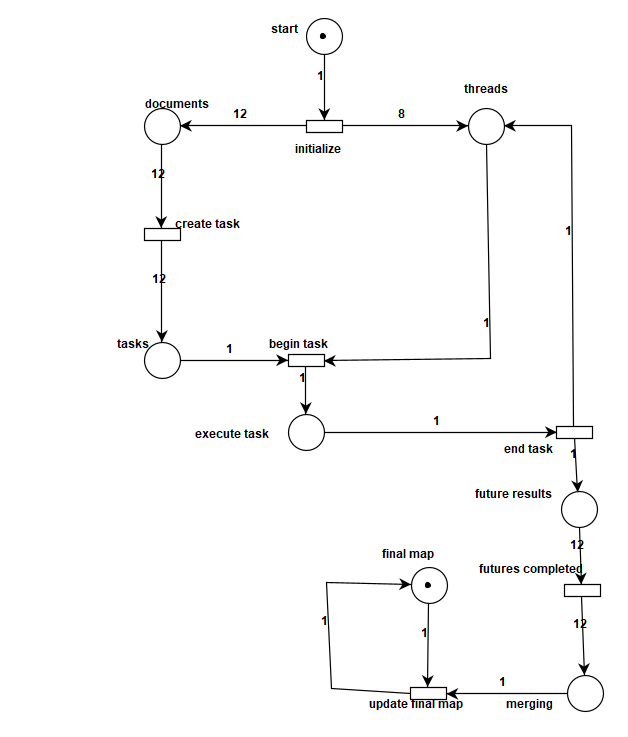
\includegraphics[width=120mm]{img/Petri net - Task frameworks.png}
    \label{fig:task_petri}
\end{figure}
\begin{warn}[NOTA:]
Al fine di astrarre il funzionamento del sistema, si assume per semplicità di utilizzare 8 thread e un numero di file PDF pari a 12. Non è possibile specificare valori generici sul peso degli archi, per cui non è possibile testare esaustivamente tutti gli scenari, anche a causa di quanto computazionalmente sarebbe dispendioso il processo.
\end{warn}
Quando la computazione di un task termina, il token del thread utilizzato ritorna nella piazza \textit{threads}.\newline
I token cominciano quindi ad accumularsi nella piazza \textit{future results} e solo una volta che tutti i task saranno stati processati verrà abilitata la transizione \textit{futures completed}.\newline
Tutti i token vengono quindi spostati nella piazza \textit{merging} e potrà iniziare la fase di merge.\newline
La piazza \textit{final map} rappresenta l'accesso alla struttura finale, che avviene in modo sequenziale.
